\documentclass[11pt,a4paper]{article}

% Packages
\usepackage{amsmath}
\usepackage{amssymb}
\usepackage{amsthm}
\usepackage[margin=1in]{geometry}
\usepackage{enumitem}
\usepackage{tikz}
\usepackage{pgfplots}
\usepackage{xcolor}
\pgfplotsset{compat=1.18}

% Custom commands
\newcommand{\stage}[1]{\textbf{\textcolor{blue}{#1}}}

% Title information
\title{Exercise Sheet 3: Bifurcations\\
Question 10 - Complete Solution}
\author{Methods of Applied Mathematics}
\date{}

\begin{document}

\maketitle

\section*{Problem Statement}

Consider the system:
\begin{align*}
\dot{x} &= \rho x - \omega y + \alpha(x^2 + y^2)x \\
\dot{y} &= \omega x + \rho y + \alpha(x^2 + y^2)y
\end{align*}
for $\omega > 0$ and $\alpha > 0$, with $\rho$ allowed to vary.

\textbf{Tasks:}
\begin{enumerate}[label=(\alph*)]
\item Find any equilibria of the system and their stability
\item Determine what bifurcation occurs at the origin when $\rho = 0$
\item Express the system in polar coordinates $(x, y) = (r\cos\theta, r\sin\theta)$, derive dynamical equations for $\dot{r}$ and $\dot{\theta}$, and describe the dynamics
\item From the polar form, show that there exists a limit cycle
\item Derive the Poincaré map and verify the limit cycle
\end{enumerate}

\vspace{10pt}
\hrule
\vspace{10pt}

\section{Step 1: Find Equilibria (Part a)}

\subsection*{Set up equilibrium conditions}

For equilibria, we require $\dot{x} = 0$ and $\dot{y} = 0$:
\begin{align*}
\rho x - \omega y + \alpha(x^2 + y^2)x &= 0 \\
\omega x + \rho y + \alpha(x^2 + y^2)y &= 0
\end{align*}

\subsection*{Obvious equilibrium: Origin}

Try $(x, y) = (0, 0)$:
\begin{align*}
0 - 0 + 0 &= 0 \quad \checkmark \\
0 + 0 + 0 &= 0 \quad \checkmark
\end{align*}

Therefore:
\[
\boxed{(x^*, y^*) = (0, 0) \text{ is an equilibrium for all } \rho}
\]

\subsection*{Search for other equilibria}

Rewrite equations:
\begin{align*}
x[\rho + \alpha(x^2 + y^2)] &= \omega y \\
y[\rho + \alpha(x^2 + y^2)] &= -\omega x
\end{align*}

Let $r^2 = x^2 + y^2$. Multiply first by $x$, second by $y$, and add:
\begin{align*}
x^2[\rho + \alpha r^2] + y^2[\rho + \alpha r^2] &= \omega xy - \omega xy = 0 \\
r^2[\rho + \alpha r^2] &= 0
\end{align*}

Either $r = 0$ (origin) or $\rho + \alpha r^2 = 0$.

For real equilibria beyond origin: $r^2 = -\frac{\rho}{\alpha}$

Since $\alpha > 0$ and $r^2 \geq 0$, this requires $\rho \leq 0$.

The hint suggests we'll understand this better in polar coordinates (part c).

\subsection*{XYZ Analysis}

\begin{itemize}[leftmargin=*]
\item \stage{STAGE X (What we found):} Origin always an equilibrium. For $\rho < 0$, hints of circular equilibria at radius $r = \sqrt{-\rho/\alpha}$.

\item \stage{STAGE Y (Why polar coordinates):} The term $x^2 + y^2 = r^2$ appears repeatedly. The system has rotational symmetry - rotating the plane doesn't change the equations. Polar coordinates will exploit this symmetry.

\item \stage{STAGE Z (Next step):} Analyze origin stability first, then transform to polar coordinates to fully understand the system.
\end{itemize}

\vspace{10pt}
\hrule
\vspace{10pt}

\section{Step 2: Stability of Origin}

\subsection*{Jacobian at origin}

For $f(x,y) = \rho x - \omega y + \alpha(x^2+y^2)x$ and $g(x,y) = \omega x + \rho y + \alpha(x^2+y^2)y$:

At $(0,0)$:
\[
J(0,0) = \begin{pmatrix}
\rho & -\omega \\
\omega & \rho
\end{pmatrix}
\]

\subsection*{Eigenvalues}

Characteristic equation: $\lambda^2 - 2\rho\lambda + (\rho^2 + \omega^2) = 0$

\[
\lambda = \frac{2\rho \pm \sqrt{4\rho^2 - 4\rho^2 - 4\omega^2}}{2} = \frac{2\rho \pm 2i\omega}{2} = \rho \pm i\omega
\]

\subsection*{Stability by $\rho$}

\begin{center}
\begin{tabular}{|c|c|c|}
\hline
$\rho$ & Eigenvalues & Stability \\
\hline
$\rho < 0$ & $\text{Re}(\lambda) < 0$ & Stable spiral \\
$\rho = 0$ & $\lambda = \pm i\omega$ & Neutral \\
$\rho > 0$ & $\text{Re}(\lambda) > 0$ & Unstable spiral \\
\hline
\end{tabular}
\end{center}

\subsection*{XYZ Analysis}

\begin{itemize}[leftmargin=*]
\item \stage{STAGE X (What we found):} Complex eigenvalues $\lambda = \rho \pm i\omega$ for all $\rho$. Real part equals $\rho$, determining stability.

\item \stage{STAGE Y (Why complex):} The Jacobian $J = \rho I + \omega R$ where $R = \begin{psmallmatrix} 0 & -1 \\ 1 & 0 \end{psmallmatrix}$ is a rotation matrix. This combines radial growth/decay ($\rho$) with rotation ($\omega$).

\item \stage{STAGE Z (What this means):} At $\rho = 0$, eigenvalues cross imaginary axis - Hopf bifurcation signature. Parameter $\rho$ controls stability, $\omega$ controls rotation frequency.
\end{itemize}

\vspace{10pt}
\hrule
\vspace{10pt}

\section{Step 3: Identify Hopf Bifurcation (Part b)}

\subsection*{Verify Hopf conditions at $\rho = 0$}

\textbf{(B1)} Equilibrium exists: $(0,0)$ exists for all $\rho$ ✓

\textbf{(B2)} Purely imaginary eigenvalues: At $\rho=0$, $\lambda = \pm i\omega$ ✓

\textbf{(G1)} Imaginary part nonzero: $\omega > 0$ (given) ✓

\textbf{(G2)} Transverse crossing: $\frac{d(\text{Re}(\lambda))}{d\rho} = 1 \neq 0$ ✓

\subsection*{Conclusion}

\[
\boxed{\text{HOPF BIFURCATION at } \rho = 0}
\]

\subsection*{XYZ Analysis}

\begin{itemize}[leftmargin=*]
\item \stage{STAGE X (What we verified):} All four Hopf conditions hold at $\rho = 0$.

\item \stage{STAGE Y (Why Hopf):} Complex eigenvalues cross imaginary axis (not real axis like fold/transcritical/pitchfork). This creates periodic orbits, not just equilibria. The sign of $\alpha > 0$ will determine if the bifurcation is supercritical (stable limit cycle) or subcritical (unstable limit cycle).

\item \stage{STAGE Z (What to expect):} Hopf bifurcation creates a limit cycle - periodic orbit. Polar coordinates will reveal its radius and stability.
\end{itemize}

\vspace{10pt}
\hrule
\vspace{10pt}

\section{Step 4: Transform to Polar Coordinates (Part c)}

\subsection*{Polar relations}

\begin{align*}
x = r\cos\theta, \quad y = r\sin\theta, \quad r^2 = x^2 + y^2
\end{align*}

\subsection*{Derive $\dot{r}$}

From $r^2 = x^2 + y^2$:
\[
2r\dot{r} = 2x\dot{x} + 2y\dot{y} \quad \Rightarrow \quad \dot{r} = \frac{x\dot{x} + y\dot{y}}{r}
\]

Substitute the original equations:
\begin{align*}
\dot{r} &= \frac{x[\rho x - \omega y + \alpha r^2 x] + y[\omega x + \rho y + \alpha r^2 y]}{r} \\
&= \frac{\rho x^2 - \omega xy + \omega xy + \rho y^2 + \alpha r^2(x^2 + y^2)}{r} \\
&= \frac{\rho(x^2+y^2) + \alpha r^2 \cdot r^2}{r} \\
&= \frac{\rho r^2 + \alpha r^4}{r}
\end{align*}

\[
\boxed{\dot{r} = r(\rho + \alpha r^2)}
\]

\subsection*{Derive $\dot{\theta}$}

From $\theta = \arctan(y/x)$:
\[
\dot{\theta} = \frac{x\dot{y} - y\dot{x}}{x^2 + y^2}
\]

Substitute:
\begin{align*}
\dot{\theta} &= \frac{x[\omega x + \rho y + \alpha r^2 y] - y[\rho x - \omega y + \alpha r^2 x]}{r^2} \\
&= \frac{\omega x^2 + \rho xy + \alpha r^2 xy - \rho xy + \omega y^2 - \alpha r^2 xy}{r^2} \\
&= \frac{\omega(x^2 + y^2)}{r^2}
\end{align*}

\[
\boxed{\dot{\theta} = \omega}
\]

\subsection*{Polar system}

\[
\boxed{
\begin{cases}
\dot{r} = r(\rho + \alpha r^2) \\
\dot{\theta} = \omega
\end{cases}
}
\]

\subsection*{XYZ Analysis of Polar Form}

\begin{itemize}[leftmargin=*]
\item \stage{STAGE X (What we derived):} Complete decoupling! The radial equation is autonomous (doesn't depend on $\theta$), and the angular equation is constant.

\item \stage{STAGE Y (Why this works):} Rotational symmetry becomes explicit:
\begin{itemize}
\item $\dot{\theta} = \omega$: All points rotate at same angular velocity, independent of radius
\item $\dot{r} = r(\rho + \alpha r^2)$: Radial dynamics independent of angle
\item The radial equation is essentially 1D: $\dot{r} = \rho r + \alpha r^3$
\end{itemize}

\item \stage{STAGE Z (What this reveals):}
\begin{itemize}
\item \textbf{Angular motion}: Constant counterclockwise rotation with period $T = 2\pi/\omega$
\item \textbf{Radial motion}: Growth if $\rho + \alpha r^2 > 0$, decay if $<0$, constant if $=0$
\item Trajectories are spirals: rotating while moving radially
\item Equilibrium of radial equation ($\dot{r}=0$) gives \textit{circular orbit} in full system
\end{itemize}
\end{itemize}

\vspace{10pt}
\hrule
\vspace{10pt}

\section{Step 5: Find Limit Cycle from Radial Equation (Part d)}

\subsection*{Equilibria of radial system}

From $\dot{r} = r(\rho + \alpha r^2) = 0$:

\textbf{Equilibrium 1:} $r = 0$

\textbf{Equilibrium 2:} $\rho + \alpha r^2 = 0$
\[
r^2 = -\frac{\rho}{\alpha}
\]

Since $\alpha > 0$ and $r \geq 0$:
\begin{itemize}
\item For $\rho > 0$: No real solution (only origin)
\item For $\rho = 0$: $r = 0$ only
\item For $\rho < 0$: $r_* = \sqrt{-\rho/\alpha}$ exists
\end{itemize}

\subsection*{Stability analysis}

Compute $\frac{d\dot{r}}{dr} = \rho + 3\alpha r^2$

\textbf{At $r = 0$:}
\[
\frac{d\dot{r}}{dr}\bigg|_0 = \rho
\]

\begin{itemize}
\item $\rho < 0$: Stable
\item $\rho = 0$: Neutral (bifurcation)
\item $\rho > 0$: Unstable
\end{itemize}

\textbf{At $r_* = \sqrt{-\rho/\alpha}$ (for $\rho < 0$):}

Since $\alpha r_*^2 = -\rho$:
\[
\frac{d\dot{r}}{dr}\bigg|_{r_*} = \rho + 3\alpha r_*^2 = \rho + 3(-\rho) = -2\rho
\]

For $\rho < 0$: $-2\rho > 0$ → \textbf{UNSTABLE}

\subsection*{Phase line for radial equation}

\textbf{For $\rho < 0$:}

\begin{center}
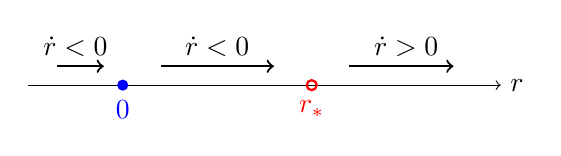
\begin{tikzpicture}[scale=1.2]
\draw[->] (0,0) -- (5,0) node[right] {$r$};
\filldraw[blue] (1,0) circle (1.5pt) node[below=2pt] {$0$};
\draw[red, thick] (3,0) circle (1.5pt) node[below=2pt] {$r_*$};
\draw[->, thick] (0.3,0.2) -- (0.8,0.2);
\draw[->, thick] (1.4,0.2) -- (2.6,0.2);
\draw[->, thick] (3.4,0.2) -- (4.5,0.2);
\node[above] at (0.5,0.2) {$\dot{r}<0$};
\node[above] at (2,0.2) {$\dot{r}<0$};
\node[above] at (4,0.2) {$\dot{r}>0$};
\end{tikzpicture}
\end{center}

Flow: $0 < r < r_*$ flows left (toward 0), $r > r_*$ flows right (to $\infty$)

\textbf{For $\rho > 0$:}

\begin{center}
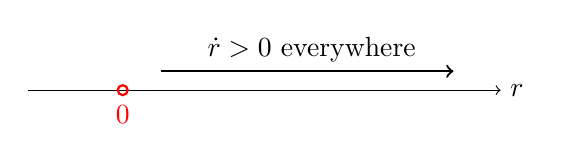
\begin{tikzpicture}[scale=1.2]
\draw[->] (0,0) -- (5,0) node[right] {$r$};
\draw[red, thick] (1,0) circle (1.5pt) node[below=2pt] {$0$};
\draw[->, thick] (1.4,0.2) -- (4.5,0.2);
\node[above] at (3,0.2) {$\dot{r}>0$ everywhere};
\end{tikzpicture}
\end{center}

All $r > 0$ flows right (to $\infty$)

\subsection*{Identify bifurcation in radial system}

The radial equation $\dot{r} = \rho r + \alpha r^3$ exhibits a bifurcation at $\rho = 0$:

\begin{itemize}
\item For $\rho < 0$: Two equilibria (origin stable, $r_*$ unstable)
\item For $\rho = 0$: One equilibrium (origin)
\item For $\rho > 0$: One equilibrium (origin unstable)
\end{itemize}

This resembles a transcritical bifurcation in the 1D radial system.

\subsection*{Limit cycle interpretation}

In the radial system, $r = r_*$ is an equilibrium for $\rho < 0$. In the full 2D system:

\begin{itemize}
\item $\dot{r} = 0$ at $r = r_*$: radius constant
\item $\dot{\theta} = \omega \neq 0$: angle increases
\end{itemize}

Therefore, trajectories at $r = r_*$ move along a circle of radius $r_*$ at constant angular velocity.

\[
\boxed{\text{Limit cycle: } x^2 + y^2 = r_*^2 = -\frac{\rho}{\alpha} \text{ for } \rho < 0}
\]

This is an \textbf{unstable limit cycle} (since $r_*$ is unstable in radial equation).

\subsection*{Subcritical Hopf bifurcation}

With $\alpha > 0$:

\begin{itemize}
\item For $\rho < 0$: Stable origin, unstable limit cycle at $r_* = \sqrt{-\rho/\alpha}$
\item At $\rho = 0$: Limit cycle shrinks to origin
\item For $\rho > 0$: Unstable origin, no limit cycle
\end{itemize}

This is a \textbf{SUBCRITICAL HOPF BIFURCATION}.

\subsection*{XYZ Analysis of Limit Cycle}

\begin{itemize}[leftmargin=*]
\item \stage{STAGE X (What we found):} For $\rho < 0$, an unstable circular limit cycle exists at radius $r_* = \sqrt{-\rho/\alpha}$. It disappears at $\rho = 0$.

\item \stage{STAGE Y (Why unstable):} The radial equilibrium $r_*$ has $d\dot{r}/dr = -2\rho > 0$ for $\rho < 0$, making it unstable:
\begin{itemize}
\item Perturbations inward ($r < r_*$): $\dot{r} < 0$, flows toward origin (away from $r_*$)
\item Perturbations outward ($r > r_*$): $\dot{r} > 0$, flows to infinity (away from $r_*$)
\end{itemize}
The limit cycle repels trajectories on both sides.

With $\alpha > 0$, the cubic term $\alpha r^3$ \textit{amplifies} rather than damps large-amplitude motion, creating subcritical (unstable) behavior.

\item \stage{STAGE Z (What this means physically):} Subcritical Hopf bifurcations are dangerous in applications:
\begin{itemize}
\item For $\rho < 0$: Basin of attraction is limited to $r < r_*$. Perturbations exceeding the limit cycle lead to unbounded growth
\item At $\rho = 0$: The safety margin (limit cycle) vanishes
\item For $\rho > 0$: Even infinitesimal perturbations cause escape to infinity
\end{itemize}
This contrasts with supercritical Hopf (e.g., $\alpha < 0$), where a stable limit cycle "catches" trajectories for $\rho > 0$.
\end{itemize}

\vspace{10pt}
\hrule
\vspace{10pt}

\section{Step 6: Poincaré Map (Part e)}

\subsection*{Define Poincaré section}

Choose section $\Sigma = \{(r,\theta) : \theta = 0\}$ (positive $x$-axis).

A point on $\Sigma$ is characterized by its radius $r_n \geq 0$.

\subsection*{Derive the map}

Starting at $(r_n, 0)$ at time $t = 0$, we solve the polar system:

\textbf{Angular equation:}
\[
\dot{\theta} = \omega \quad \Rightarrow \quad \theta(t) = \omega t
\]

Return to section when $\theta = 2\pi$:
\[
\omega t^* = 2\pi \quad \Rightarrow \quad t^* = \frac{2\pi}{\omega}
\]

\textbf{Radial equation:}
\[
\dot{r} = r(\rho + \alpha r^2)
\]

This is separable:
\[
\frac{dr}{r(\rho + \alpha r^2)} = dt
\]

\subsection*{Integrate radial equation}

Use partial fractions:
\[
\frac{1}{r(\rho + \alpha r^2)} = \frac{1}{\rho r} - \frac{\alpha r}{\rho(\rho + \alpha r^2)}
\]

Integrate from $t = 0$ (radius $r_n$) to $t = t^*$ (radius $r_{n+1}$):
\[
\frac{1}{\rho}\log\left(\frac{r_{n+1}}{r_n}\right) - \frac{1}{2\rho}\log\left(\frac{\rho + \alpha r_{n+1}^2}{\rho + \alpha r_n^2}\right) = t^* = \frac{2\pi}{\omega}
\]

Simplify:
\[
\log\left(\frac{r_{n+1}}{r_n}\right) - \frac{1}{2}\log\left(\frac{\rho + \alpha r_{n+1}^2}{\rho + \alpha r_n^2}\right) = \frac{2\pi\rho}{\omega}
\]

\[
\log\left(\frac{r_{n+1}}{\sqrt{\rho + \alpha r_{n+1}^2}}\right) - \log\left(\frac{r_n}{\sqrt{\rho + \alpha r_n^2}}\right) = \frac{2\pi\rho}{\omega}
\]

Define $\phi(r) = \log\left(\frac{r}{\sqrt{\rho + \alpha r^2}}\right)$:
\[
\phi(r_{n+1}) - \phi(r_n) = \frac{2\pi\rho}{\omega}
\]

\[
\boxed{r_{n+1} = P(r_n) \text{ given implicitly by } \phi(r_{n+1}) = \phi(r_n) + \frac{2\pi\rho}{\omega}}
\]

\subsection*{Fixed points of Poincaré map}

Fixed point $r^*$: $P(r^*) = r^*$

This requires:
\[
\phi(r^*) = \phi(r^*) + \frac{2\pi\rho}{\omega}
\]

Only possible if $\frac{2\pi\rho}{\omega} = 0$, i.e., $\rho = 0$.

For $\rho \neq 0$, fixed points come from:
\[
\phi(r^*) - \phi(r^*) = 0 = \frac{2\pi\rho}{\omega}
\]

Wait, let me reconsider. A fixed point means $r_{n+1} = r_n = r^*$. Substituting into the radial equation:

During the time interval $[0, t^*]$, if $r$ remains constant, then $\dot{r} = 0$ always, which requires:
\[
r^*(\rho + \alpha r^{*2}) = 0
\]

So fixed points are $r^* = 0$ or $r^* = \sqrt{-\rho/\alpha}$ (for $\rho < 0$).

\subsection*{Stability of fixed points}

Compute $\frac{dP}{dr}$ at fixed point. For $\dot{r} = r(\rho + \alpha r^2)$:

\[
\frac{dr_{n+1}}{dr_n} = \exp\left(\int_0^{t^*} \frac{\partial \dot{r}}{\partial r} dt\right) = \exp\left(\int_0^{t^*} (\rho + 3\alpha r^2) dt\right)
\]

For $r = r^*$ constant:
\[
\frac{dP}{dr}\bigg|_{r^*} = \exp\left((\rho + 3\alpha r^{*2}) \cdot \frac{2\pi}{\omega}\right)
\]

\textbf{At $r^* = 0$:}
\[
\frac{dP}{dr}\bigg|_0 = \exp\left(\frac{2\pi\rho}{\omega}\right)
\]

\begin{itemize}
\item $\rho < 0$: $|dP/dr| < 1$ → Stable
\item $\rho > 0$: $|dP/dr| > 1$ → Unstable
\end{itemize}

\textbf{At $r^* = \sqrt{-\rho/\alpha}$ (for $\rho < 0$):}

Since $\rho + 3\alpha r^{*2} = \rho - 3\rho = -2\rho$:
\[
\frac{dP}{dr}\bigg|_{r^*} = \exp\left(\frac{-4\pi\rho}{\omega}\right) = \exp\left(\frac{4\pi|\rho|}{\omega}\right) > 1
\]

Unstable fixed point.

\subsection*{Verify limit cycle existence}

The Poincaré map analysis confirms:

\begin{itemize}
\item For $\rho < 0$: Two fixed points - $r=0$ (stable) and $r^* = \sqrt{-\rho/\alpha}$ (unstable)
\item The unstable fixed point corresponds to the unstable limit cycle in the continuous system
\item Period of limit cycle: $T = 2\pi/\omega$
\end{itemize}

\[
\boxed{\text{Limit cycle verified via Poincaré map}}
\]

\subsection*{XYZ Analysis of Poincaré Map}

\begin{itemize}[leftmargin=*]
\item \stage{STAGE X (What we derived):} The Poincaré map $P: r_n \mapsto r_{n+1}$ reduces the 2D continuous system to a 1D discrete map. Fixed points of $P$ correspond to periodic orbits.

\item \stage{STAGE Y (Why this works):} The section $\theta = 0$ is transverse to the flow (since $\dot{\theta} = \omega \neq 0$). Every trajectory crosses it periodically. The map encodes one full revolution:
\begin{itemize}
\item Start at radius $r_n$
\item Flow for time $t^* = 2\pi/\omega$ (one full rotation)
\item Return to section at radius $r_{n+1}$
\end{itemize}

Fixed points ($r_{n+1} = r_n$) mean the trajectory returns to the same radius after one revolution - a periodic orbit. The derivative $dP/dr$ determines stability: $|dP/dr| < 1$ means nearby orbits converge, $|dP/dr| > 1$ means they diverge.

\item \stage{STAGE Z (What this reveals):} The Poincaré map confirms our continuous analysis:
\begin{itemize}
\item Origin: Fixed point, stable for $\rho < 0$, unstable for $\rho > 0$
\item Limit cycle: Fixed point at $r^* = \sqrt{-\rho/\alpha}$ for $\rho < 0$, unstable
\item Period: $T = 2\pi/\omega$, independent of radius
\end{itemize}

The Poincaré map is a powerful tool: it reduces dimension (2D → 1D), converts continuous → discrete, and preserves essential dynamics (fixed points ↔ periodic orbits, stability preserved).
\end{itemize}

\vspace{10pt}
\hrule
\vspace{10pt}

\section{Summary}

\subsection*{Complete bifurcation picture}

\textbf{System:}
\[
\dot{x} = \rho x - \omega y + \alpha(x^2 + y^2)x, \quad \dot{y} = \omega x + \rho y + \alpha(x^2 + y^2)y
\]

\textbf{Polar form:}
\[
\dot{r} = r(\rho + \alpha r^2), \quad \dot{\theta} = \omega
\]

\textbf{Equilibria and limit cycles:}

\begin{center}
\begin{tabular}{|c|l|}
\hline
\textbf{Parameter} & \textbf{Behavior} \\
\hline
$\rho < 0$ & Stable spiral at origin \\
& Unstable limit cycle at $r = \sqrt{-\rho/\alpha}$ \\
\hline
$\rho = 0$ & Neutral spiral (Hopf bifurcation) \\
\hline
$\rho > 0$ & Unstable spiral at origin \\
& No limit cycle (trajectories escape) \\
\hline
\end{tabular}
\end{center}

\textbf{Bifurcation type:}

\[
\boxed{\text{SUBCRITICAL HOPF BIFURCATION}}
\]

With $\alpha > 0$, the cubic nonlinearity amplifies large-amplitude motion, creating an unstable limit cycle for $\rho < 0$ that shrinks to zero at $\rho = 0$ and disappears for $\rho > 0$.

\textbf{Key insights:}
\begin{itemize}
\item Polar coordinates reveal the system's rotational symmetry
\item Radial equation is 1D, making analysis tractable
\item Limit cycle is a circle with constant rotation
\item Poincaré map confirms limit cycle existence and stability
\item Subcritical bifurcation creates dangerous dynamics (limited basin of attraction)
\end{itemize}

\end{document}
